% !TeX root=abs_formeln.tex

\begin{equation}\label{eq:schwingung:frequenz}
f = \frac{n}{t} = \frac{1}{T}
\end{equation}

\subsection{Harmonische Schwingung}
$\varphi = \text{Phasenwinkel}$, $\SI{360}{\degree} \hat{=} 2\pi $

\subsubsection{Winkelgeschwindigkeit $\omega$}
\begin{equation}\label{eq:schwingung:winkelgeschwindigkeit}
\omega = \frac{\varphi}{t} = \frac{2 \pi}{T} = 2 \pi f
\end{equation}

\subsubsection{Elongation $s$}
\begin{equation}\label{eq:schwingung:elongation}
s = r \cdot \sin \varphi \quad \hat{s} = r
\end{equation}

\subsubsection{Zeit-Weg-Gesetz}
\begin{equation}\label{eq:schwingung:t:s:gesetz}
s(t) = \hat{s}\cdot\sin(\omega\cdot t)
\end{equation}

\subsubsection{Zeit-Geschwindigkeits-Gesetz}
\begin{equation}\label{eq:schwingung:t:v:gesetz}
v(t) = \omega \cdot \hat{s} \cdot \cos(\omega \cdot t)
\end{equation}

\subsubsection{Zeit-Beschleunigungs-Gesetz}
\begin{equation}\label{eq:schwingung:t:a:gesetz}
a(t) = - \omega^2 \cdot \hat{s} \cdot \sin(\omega \cdot t)
\end{equation}

\begin{equation}\label{eq:schwingung:beschleunigung:allgemein}
a(t) = \dot{v}(t) = \ddot{s}(t)
\end{equation}

\subsubsection{Elongations-Kraft-Gesetz}
(Bedingung für harmonische Schwingung)
\begin{equation}\label{eq:schwingung:ruecktreibende:kraft}
F = - D \cdot s
\end{equation}
mit Richtgröße $D$
\begin{equation}\label{eq:schwingung:richtgroesse}
D = m \cdot \omega^2
\end{equation}
liefert die Periodendauer
\begin{equation}\label{eq:schwingung:periodendauer}
T = 2\pi \sqrt{\frac{m}{D}}
\end{equation}

\subsubsection{Energie einer ungedämpften harmonischen Schwingung}
\begin{equation}\label{eq:energie:ungedaempfte;harmonische:schwingung}
\begin{split}
W &= W_{Elong} + W_B \\
   &= \frac{1}{2} D \cdot s^2 + \frac{1}{2} m \cdot v^2 = \text{konst.}
\end{split}
\end{equation}

\subsubsection{Schwingung des Fadenpendels}
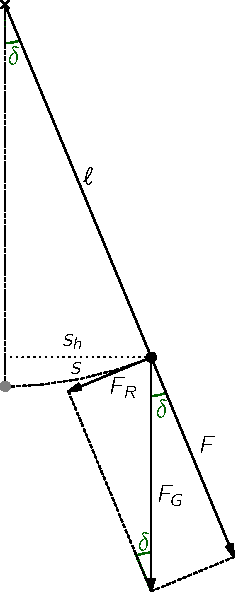
\includegraphics[width=.35\linewidth]{fadenpendel}
\hfill
\begin{minipage}[b]{.6\linewidth}
Auslenkung des Pendels: $s$ 
\begin{equation}\label{eq:fadenpendel:auslenkung}
s = \ell\cdot\delta
\end{equation}

\begin{equation}\label{eq:fadenpendel:winkel}
\sin\delta = \frac{s_h}{\ell} \approx \frac{s}{\ell} 
\end{equation}

\begin{equation}\label{eq:fadenpendel:winkel:kraefte}
\sin\delta = \frac{F_R}{F_G}
\end{equation}

\begin{equation}\label{eq:fadenpendel:ruecktreibende:kraft}
F_R = \frac{m \cdot g \cdot s}{\ell}
\end{equation}

\begin{equation}\label{eq:fadenpendel:richtgroesse}
D = \frac{m \cdot g}{\ell}
\end{equation}

\begin{equation}\label{eq:fadenpendel:periodendauer}
T = 2 \pi\sqrt{\frac{\ell}{g}}
\end{equation}
\end{minipage}

\subsubsection{Elektromagnetischer Schwingkreis}
\begin{equation}\label{eq:elektromagnetischer:schwingkreis:ladung}
Q = \hat{Q}\cos(\omega \cdot t)\\
\end{equation}

\begin{equation}\label{eq:elektromagnetischer:schwingkreis:spannung}
U = \hat{U}\cos(\omega \cdot t)\\
\end{equation}

\begin{equation}\label{eq:elektromagnetischer:schwingkreis:stromstaerke}
I = - \hat{I}\sin(\omega \cdot t)
\end{equation}

\begin{equation}\label{eq:elektromagnetischer:schwingkreis:winkelgeschwindigkeit}
\omega = \frac{1}{\sqrt{L \cdot C}}
\end{equation}

\begin{equation}\label{eq:elektromagnetischer:schwingkreis:maximale:stromstaerke}
\hat{I} = \frac{\hat{U} \cdot C}{\sqrt{L \cdot C}}
\end{equation}

\begin{equation}\label{eq:elektromagnetischer:schwingkreis:periodendauer}
T = 2\pi \sqrt{L \cdot C}
\end{equation}

\subsubsection{Resonanzbedingung}
\begin{equation}\label{eq:resonanzbedingung}
f = f_0 \quad\text{mit}\quad \varphi = \frac{\pi}{2}
\end{equation}

\subsubsection{Eigenschwingungen zwischen zwei festen Enden}
\begin{equation}\label{eq:eigenschwingung:laengen}
\ell = k \cdot \frac{\lambda_k}{2} \quad k = 1, 2, 3,\ldots
\end{equation}

\begin{equation}\label{eq:eigenschwingung:frequenzen}
f_k = k \cdot \frac{c}{2 \cdot \ell} \quad k = 1, 2, 3,\ldots
\end{equation}